\section{Data}
\label{sec:data}
Deze sectie bevat het EER-model voor de databank.
Eveneens bezit het ook een voorstelling van het databaseschema die dit model realiseert.

Figuur~\ref{fig:EER diagram} toont het EER-model van de databank. Om overzicht te bewaren worden de attributen die iedere entiteit bezit niet weergegeven in dit model.

\begin{figure}[H]
	\centering
	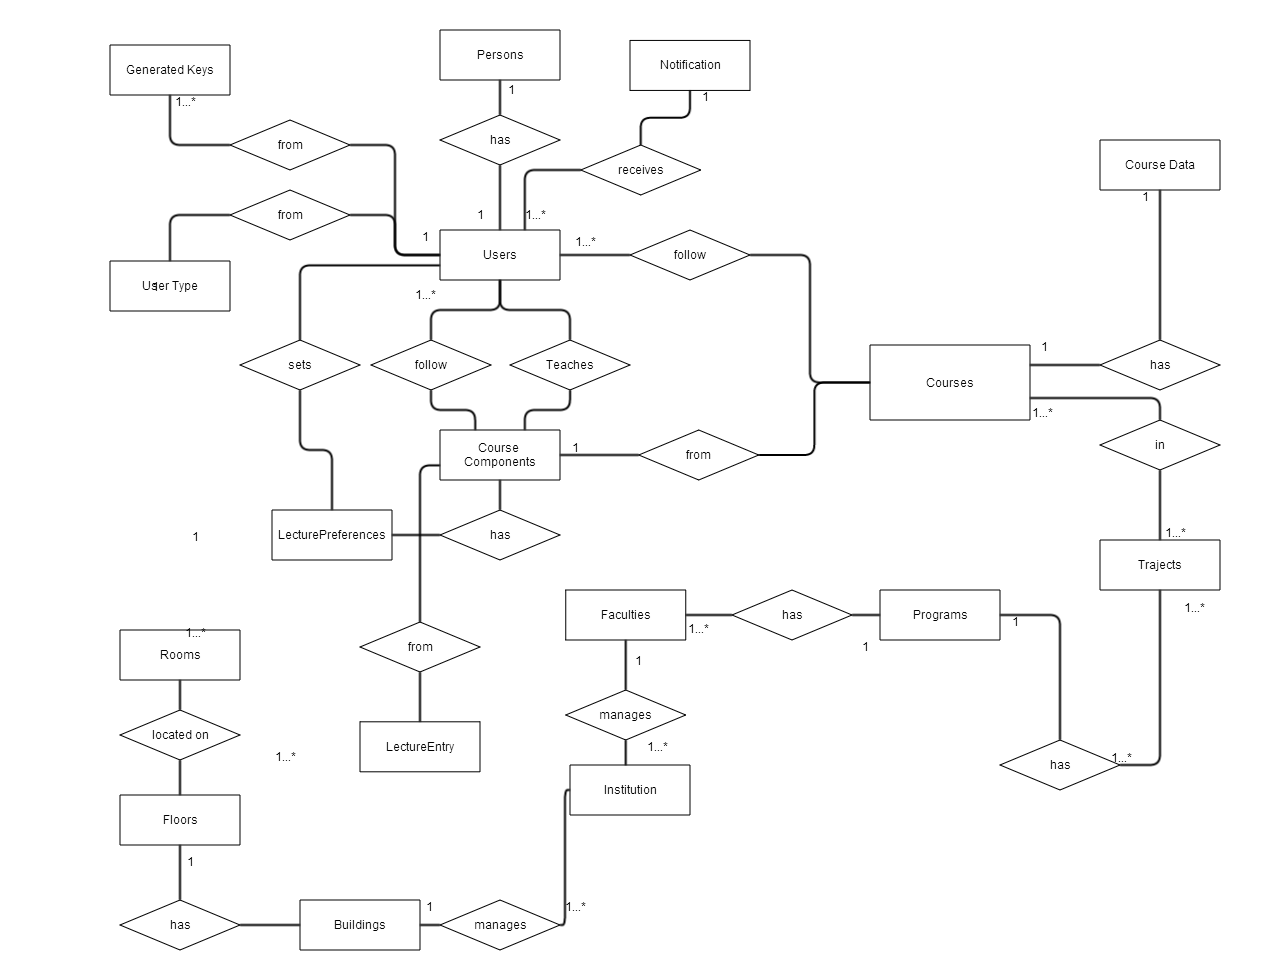
\includegraphics[scale=0.4]{img/ER4-gliffy}
	\caption{EER diagram}
	\label{fig:EER diagram}
\end{figure}

Figuren \ref{fig:db1}, \ref{fig:db2}, \ref{fig:db3} en \ref{fig:db4} tonen de huidige status van het database schema.

\begin{figure}[H]
	\centering
	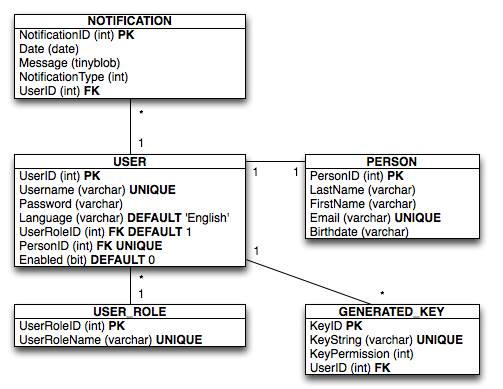
\includegraphics[scale=0.5]{design/EER/design1}
	\caption{Eerste deel van het database schema}
	\label{fig:db1}
\end{figure}

\begin{figure}[H]
	\centering
	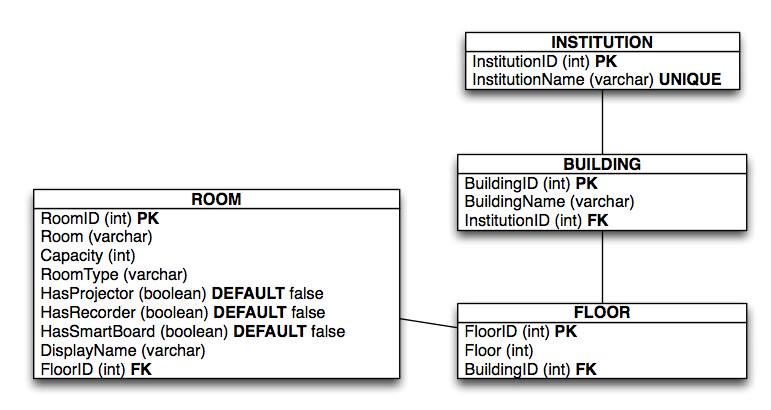
\includegraphics[scale=0.4]{design/EER/design2}
	\caption{Tweede deel van het database schema}
	\label{fig:db2}
\end{figure}

\begin{figure}[H]
	\centering
	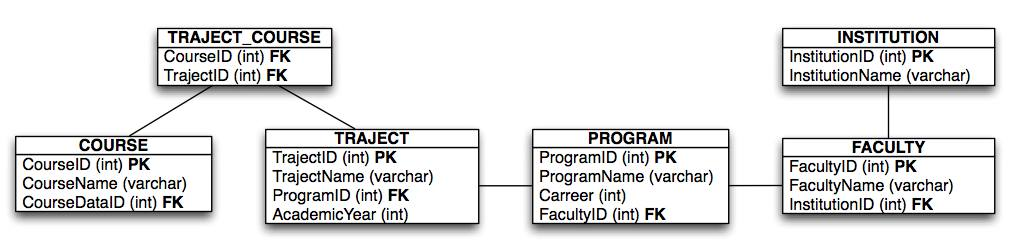
\includegraphics[scale=0.4]{design/EER/design3}
	\caption{Derde deel van het database schema}
	\label{fig:db3}
\end{figure}

\begin{figure}[H]
	\centering
	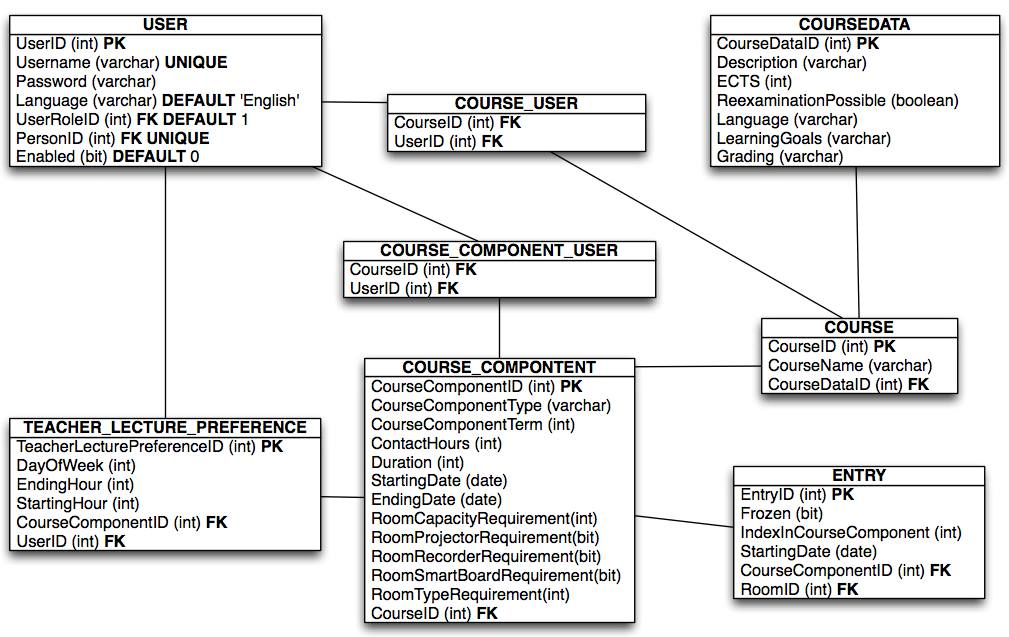
\includegraphics[scale=0.4]{design/EER/design4}
	\caption{Vierde deel van het database schema}
	\label{fig:db4}
\end{figure}